% Template for PLoS
% Version 1.0 January 2009
%
% To compile to pdf, run:
% latex plos.template
% bibtex plos.template
% latex plos.template
% latex plos.template
% dvipdf plos.template

\documentclass[10pt]{article}

% amsmath package, useful for mathematical formulas
\usepackage{amsmath}
% amssymb package, useful for mathematical symbols
\usepackage{amssymb}

% graphicx package, useful for including eps and pdf graphics
% include graphics with the command \includegraphics
\usepackage{graphicx}

% cite package, to clean up citations in the main text. Do not remove.
%\usepackage{cite}
\usepackage[round,sort]{natbib}

\usepackage{color} 

% Use doublespacing - comment out for single spacing
%\usepackage{setspace} 
%\doublespacing


% Text layout
\topmargin 0.0cm
\oddsidemargin 0.5cm
\evensidemargin 0.5cm
\textwidth 16cm 
\textheight 21cm

% Bold the 'Figure #' in the caption and separate it with a period
% Captions will be left justified
\usepackage[labelfont=bf,labelsep=period,justification=raggedright]{caption}

% Use the PLoS provided bibtex style
%\bibliographystyle{plos2009}
\bibliographystyle{abbrvnat}

% Remove brackets from numbering in List of References
\makeatletter
\renewcommand{\@biblabel}[1]{\quad#1.}
\makeatother


% Leave date blank
\date{}

\pagestyle{myheadings}
%% ** EDIT HERE **
\definecolor{linkcol}{RGB}{0,0,238}

% \usepackage[english]{babel}
\usepackage[utf8]{inputenc}
\usepackage{hyperref}
\usepackage[hypcap]{caption}

%% For hyperref
\hypersetup{
    breaklinks,
    baseurl       = http://,
    colorlinks    = true,
    linkcolor     = linkcol,
    citecolor     = linkcol,
    pdfborder     = 0 0 0
}

%% ** EDIT HERE **
%% PLEASE INCLUDE ALL MACROS BELOW

%% END MACROS SECTION

\begin{document}

% Title must be 150 characters or less
\begin{flushleft}
{\Large
\textbf{Phylogenetic footprinting, a pipeline for motif identification in \textit{Paramecium}}
}
% Insert Author names, affiliations and corresponding author email.
\\
Matthias Grenié$^{1}$, 
Jean-François Goût$^{2}$, 
Michael Lynch$^{2}$
\\
\bf{1} Départment de Biologie, École Normale Supérieure de Lyon, Lyon, France
\\
\bf{2} Biology Department, Indiana University, IN, United States of America
\\
\end{flushleft}

% Please keep the abstract between 250 and 300 words
\section*{Abstract}

% Please keep the Author Summary between 150 and 200 words
% Use first person. PLoS ONE authors please skip this step. 
% Author Summary not valid for PLoS ONE submissions.  
\section*{Author Summary}

\section*{Introduction}

Structure of the introduction
\newline
\begin{itemize}
\item Whole Genome Duplications background, major evolutionary force
\item the \textit{Paramecium} project, why \textit{Paramecium} is interesting, the aurelia complex
\item Here, focusing on the computational part, developing pipeline, showed that etc.
\end{itemize}

Since Ohno first hypothesized the influence of Whole-Genome Duplications (WGD), scientists kept showing that a broad number of organisms experienced several rounds of WGD: yeast, insects, Angiosperma, Vertebrates, Salmonids, and many others. WGD are evolutionary event when the genome of a given individual is duplicated, meaning that the whole genome is in two copies, duplicated pairs of genes are \textbf{paralogs}. WGD can also occur when two closely related species hybridize and form a fertile descendant.

WGDs may be involved in many evolutive radiations as they provide the raw material to explore new evolutionary landscapes. A recent study on the horshoe crab genome underlined that WGDs may be a more common phenomenon than stated. They showed that at least a WGD occurred in this conserved lineage, thus WGDs may not be evolutionary drivers.

Still, it seems that WGDs are widespread along the tree of life and since Ohno numerous models have been developed to explain the retention rate we observe between duplicate genes (reviewed in ). Gene Balance Hypothesis is for example a well explored hypothesis in the litterature, according to this hypothesis dosage-sensitive gene are more retained because of stœchiometry issues, it would thus explain the over retention of transcription factors and multicomplexes proteins.

To understand the consequences of WGDs we have been studying various \textit{Paramecium} species. \textit{Paramecium} are a Ciliates group (See position on phylogenetic tree). Aury \textit{et al.} showed that at least three round of WGDs occured in the \textit{Paramecium} genus, two of which occured in the \textit{aurelia} complex.  In the \textit{Paramecium} genus, the \textit{aurelia} complex of species is of particular interest. Indeed, 

The diversity of the \textit{Paramecium} ciliates is well studied. We focused on four species of \textit{Paramecium}: \textit{P. biaurelia}, \textit{P. sexaurelia}, \textit{P. tetraurelia} and \textit{P. caudatum} as an outgroup (see phylogenetic tree). The three \textit{aurelia} species underwent two rounds of WGDs, WGDX (... years ago) and WGDX (... years ago).

We have shown previous the tight link between gene expression and duplicate retention among \textit{P. caudatum} and \textit{P. tetraurelia}. Highly expressed genes are more retained than low expressed genes; the regulation of gene expression thus impacts gene retention. \textit{Cis}-regulatory sequences are upstream sequences influencing downstream gene expression.

Transcription Factor Binding Sites, regulatory sequences, regulatory network?, conserved sequences, studied for a long time. Regulatory sequences <-> WGD?

Objective: detect conserved TFBS among various our species -> to identify candidates for further studies.

\textbf{Biological questions:} Do gene expression is linked, in \textit{P.}, with specific motifs? How are TFBS affected by WGD? Are they conserved among species, is this linked to expression level? Conserved among each species? Is there a bias of TFBS usage in certain species?

\section*{Methods}

Used TranslatorX, PhyML, BigFoot, MEME.

We set up a pipeline to make our analyse (Fig. ), the code is available at.

\subsection*{Genomes and Annotation}

We used annotation and sequence from our previous analyses for P. and P. etc. (see .) and the additionnal sequence of.

\subsection*{Gene families}

Looking at the phylogenetic tree of the \textit{aurelia} species, two WGDs occured at the root and affected three of our species. We have established some gene families from WGD2 using comparison, each family contains a set of orthologous genes between the four \textit{aurelia} species studied, and eventually, the paralogous gene found in each species ; at maximum the families contain 13 different genes. Those families were established previously in our team. For details in the method see

\subsection*{Upstream sequences extraction}

We considered only families with at least 4 genes. Then, using our genome assembly and annotation of each species, we extracted upstream regions, upstream of the start codon, from 15nt with a cut-off at 250nt of all genes of the family. If the upstream region of a gene overlapped with another gene we discarded the gene, if the upstream region was less than 15nt long we also discarded the gene. Considering discarded genes, we kept only families with at least 4 members in our datasets.

\subsection*{Coding Sequences extraction and alignment}

Phylogenetic footprinting requires a phylogenetic tree to weigh the evolutionary signal of given motifs. A motif conserved between two close species will have less importance than a motif conserved in two distant species. Because we are focusing on the conservation of upstream sequences we chose not to use them to avoid circularity. Instead,corresponding coding sequences (CDS) were extracted and used to model phylogenetic trees for each family. We preferred to have a gene tree over species tree, to avoid eventual inconsistencies because of gene conversion (ref. needed). See Challenges section for explanations on the use of gene tree over species tree.

CDSs in each family were aligned using TranslatorX (ref. needed) a protein-guided alignment software. The Maximum Likelihood (ML) tree was then computed using PhyML (ref. needed) default parameters.

\subsection*{Phylogenetic footprinting}

We used a phylogenetic footprinting software BigFoot (ref. needed) to detect highly conserved motifs in upstream sequences. We used 10000 burn-in cycles and 20000 cycles with a sampling rate of 1000 for the Hidden Monte-Carlo Markov Chain (HMCMC) process. BigFoot aligns the given sequences with gaps and tries to identify conserved and non-conserved regions ; it models the evolution of those regions along the phylogenetic tree assuming conserved regions evolve more slowly than non-conserved ones. At the end of the analysis BigFoot outputs an alignment of sequences used to identify slow and fast evolving regions as well as, for each nucleotide in the alignment, the posterior probability of the alignment, higher values show higher confidence in the alignment, and the phylogenetic footprinting result, higher values indicating higher posterior probability of purifying selection.

Using a phylogenetic footprinting program means we have to use a phylogenetic tree and depending on the phylogenetic tree we are using, the evolutionary signal used in the footprinting is not identical.

The species tree (see figure.) gives us the relation between all considered, accounting for the various splits between species along with WGDs. The problem is that, not all gene families follow this tree. Because of the successive round of WGDs there are several fates possible for pair of duplicate after the first WGD. Some of these genes may cluster together in the same leaves, if the pairs diverge between species ; another possible outcome is the subfunctionnalization of each gene before the second WGD, meaning before the speciation of the \textit{aurelia} complex, thus genes from different species would cluster together in a phylogenetic tree ; or even a combination of the previous outcome and gene conversion, leading paralogs to recombine in a copy-paste way, changing dramatically the gene tree.

Using these scores we detected motifs of at least 6 nucleotides long, alignment score over 0.8 and phylogenetic score over 0.9. Because of the known biological nature of Transcription Factor Binding Sites, we allowed for a "gap" in motifs of 2 nucleotide, so that the scores could drop under the thresholds in those gaps.

BigFoot does not output directly identified motifs, instead it produces two files with an alignment of the sequences and associated phylogenetic and alignment scores, as explained above.

Transcription factor binding sites are known to be generally conserved but degenerate on certain positions. For example, ... showed that this motif was conserved ....NN... with two highly variable positions (denoted by "N", meaning "A", "T", "C" or "G" using IUPAC notation). Thus, to seek biologically relevant motifs, we had to take into account that in the middle of motifs, the phylogenetic score could drop on several positions, before rising again.

To answer this problem we use a sliding window method of 8 nucleotides in our analysis: for each family, we looked at the scores of 8 nucleotides at the time and slide along the sequences. If the window contained at least 6 bases with scores above our thresholds, we would retain this motif. Then, from this particular region we would try to extend the sequence by adding adjacent nucleotides with good scores.

\subsection*{Comparison with MEME}

To check our predictions and assess the conservation of found motifs, we compared motifs prediction with those of MEME, a widely used \textit{ab initio} motif finding tools. It searches for statistically significant motifs, with a gap-less, local multi-alignment system.

MEME was shown to have a very high False Positive Rate of the discovery (Ref. needed). That is why many studies combine multiple motif detection tools (Ref. needed). In our case, MEME is of particular interest as it obtains motifs using a totally different method from BigFoot.

To assess the relevance of motifs found from BigFoot's outputs, we compared them to a well-known motif finding program: MEME. For each family we identified overlapping motifs between MEME and BigFoot. We computed an overlapping index as follows: 
\begin{equation}
0 \leq \frac{nucleotides in common}{size of the smallest motif} \leq 1
\end{equation}
if this index was over $0.9$ we would then considered the motif as relevant.

\subsection*{Motif classification and data analysis}

All the analyses were produced using R, scatter plots and graphs were produced using the R package ggplot2.



\section*{Results}
\label{sec:Results}

From our orthologs and paralogs gene familes we had 5751 families, only 5008 gene families had at least 4 genes. We ran our pipeline on these 5008 families, to detect conserved motifs among upstream sequences of \textit{Paramecium} genomes. The pipeline was set to detect motifs, in upstream regions ranging between 15nt and 250nt (see~\nameref{sec:Methods}) , of at least 6 nucleotides with an eventual gap in conservation (see ~\autoref{fig:DegenerateMotif}) for more biological relevance.

Using BigFoot we identified 811 different motifs in 608 families. Comparing these motifs with MEME ones for partial match, only 117 unique motifs were retained. For each of these, we extracted the name of all genes containing the motif, in each species. To focus only on conserved motifs, we conserved only motifs matching in all the four species. Only 10 motifs matched these conditions. We then computed the ratio of genes containing the motif over the total number of genes (results are summed up in~\autoref{tab:Motifs}).

\section*{Future Directions}
\label{sec:Future}

We identified motifs using an automated pipeline (Fig.~\ref{fig:Pipeline}), comparing motifs identified using phylogenetic footprinting and statistical enrichment methods. We were able to dectect X motifs, associated with specific expression values and distance. Still, we plan to improve this pipeline in several ways.

After identifying motifs, we scan the entire \textit{Paramecium} genomes to find associated genes, however we only search for perfect matches. Thus, we do not take into account degenerate motifs. Thus we can miss genes that have slightly different motifs. Recently XXX showed that looking exact matches during motif identification may miss most of the signal. Indeed we have increase evidence that real motifs are most of the time degenerate and that Transcription Factor binding mostly depends on the general DNA context.

After identifying motifs, one's might want to group the motifs by similarity. We generally think about motifs as families, having specific sequences with some variation. For the moment, in our pipeline, we do not cluster motifs using "supposed" family, we consider each exact motifs as unique. However, several clustering methods exist to measure the diversity among motifs. The small sizes of motifs (about 6nt to 15nt) make these methods complicated to develop. Several methods have been implemented, but still, are not adapted for motifs and do not output families of motifs. 

Another way to think about the problem can be to cluster motifs according to features one can measure on them. For example, one can compute several statistical indexes on motifs to compare. Thus we do not need to implement a new algorithm to cluster motifs as other classical methods such as principal components analysis, hierarchal clustering or \textit{k}-means clustering can be applied. Still, these methods rely on the indexes you choose to measure, the motifs you are studying have to have well-defined clusters using those variables. We tried to cluster the studied motifs with this hierarchal clustering method (Fig.).

Several other new methods have been proposed to cluster motifs as they are, considering the sequences and the variability along each nucleotide. Some of them rely on position-specific weight matrices (PSM) which are matrices of the abundances of each base at each position. In a future improvement of the pipeline we cool try to implement such methods to reduce the redundancy of our data.

It has been proven that most motif identification tools have a high false positive discovery rate, thus, we need ways to confirm the relevance of found motifs. One way used by \citealt{liseron-monfils_promzea:_2013} is to increase the number of tools used in the pipeline, in their analysis they used MEME, BioProspector and Weeder and filtered out significant results and then only combined them. They have selected in each set, significant motifs using p-values and then only compare them. Liseron \textit{et al.} showed that by combining these tools they were able to increase the sensitivity by 22\% over the best standalone tool. Here we used MEME and BigFoot but we could include other tools in our workflow.

% Do NOT remove this, even if you are not including acknowledgments
\section*{Acknowledgments}

I would to thank my advisor Jean-François Goût for his patient and constant support, Michael Lynch for having me in his lab. More broadly, I would like to thank the whole Lynch lab team, for great scientific and non-scientific discussions.

\section*{Figure Legends}

\begin{figure}[!ht]
\begin{center}
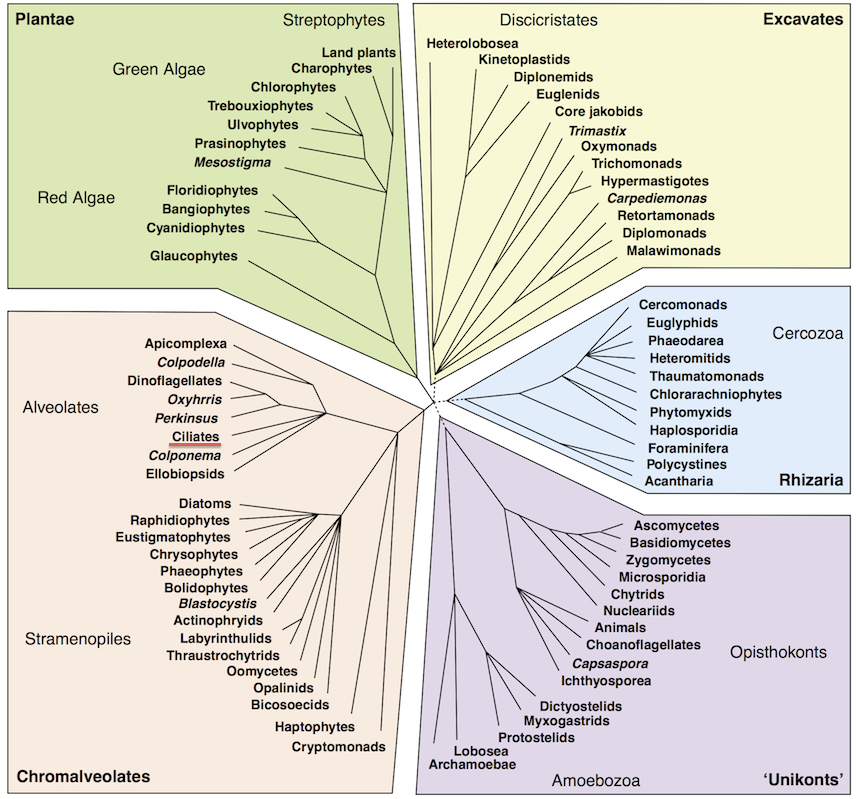
\includegraphics[scale=2.2]{Figures/TreeOfEuk.png}
\end{center}
\caption{
{\bf Phylogenetic tree of eukaryotes phylas.} The \textit{Ciliates} group, underlined in red in the figure, inside the Alveolates among the Chromoalveloates, it contains the \textit{Paramecium} genus. While the Animals (Metazoa) belong to the Opisthokonts group. From~\citep{keeling_tree_2005}
} 
\label{fig:TreeOfEuk}
\end{figure}


\begin{figure}[!ht]
\begin{center}
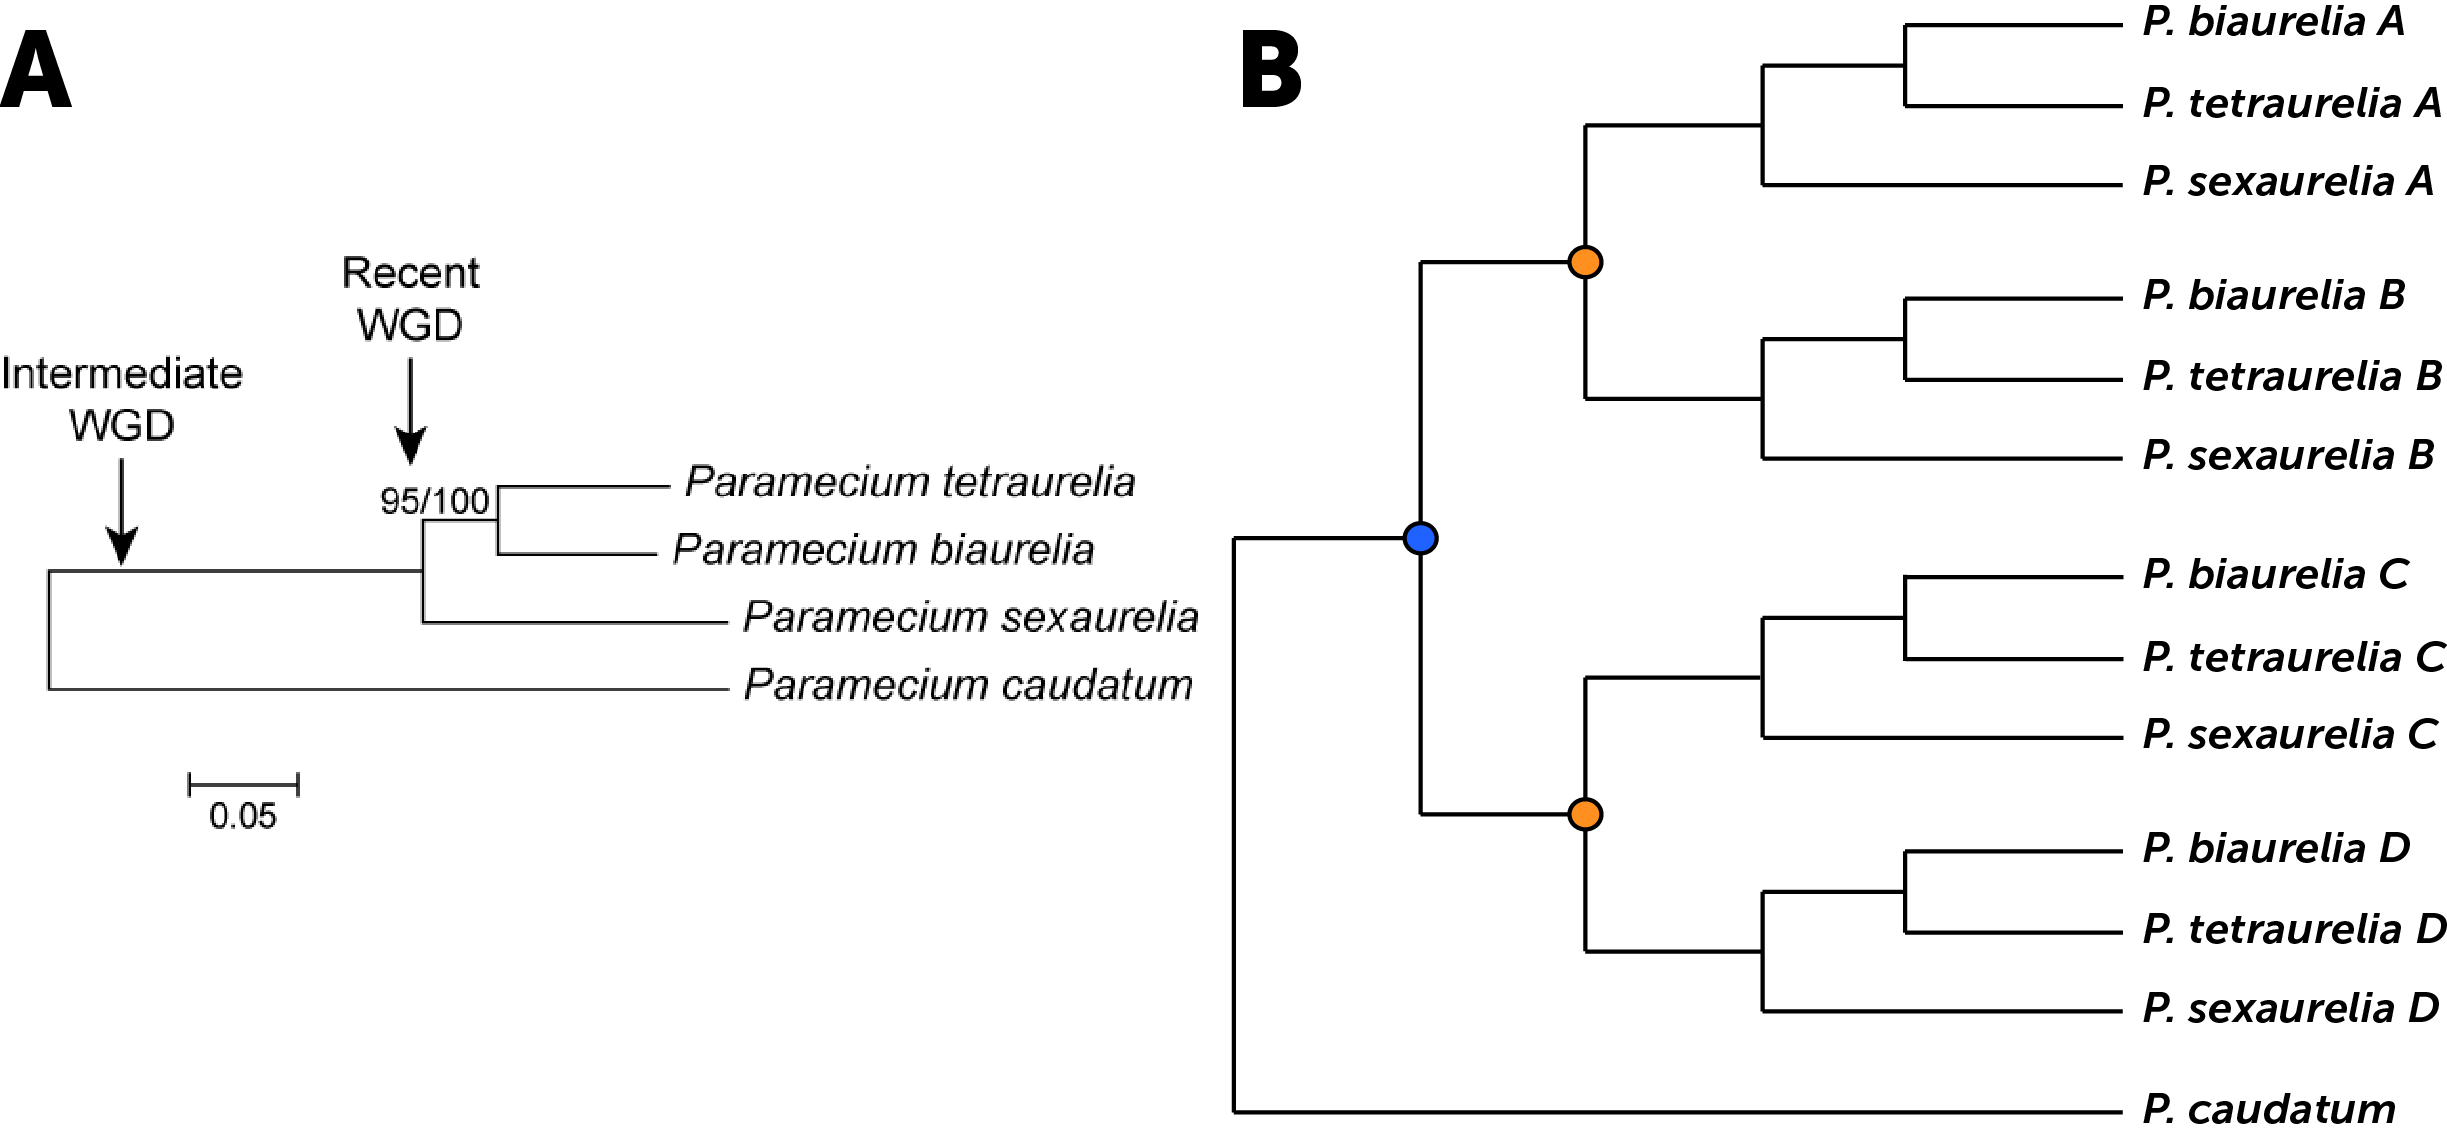
\includegraphics[scale=0.7]{Figures/SpeciesGene.png}
\end{center}
\caption{
{\bf Phylogenetic trees of \textit{Paramecium} and according gene tree.} A: \textit{Paramecium} species tree with WGD positions (Adapted from~\citealt{mcgrath_insights_2014}); B: An example of a family gene tree. A single \textit{caudatum} gene and four genes for each \textit{aurelia} species. \textit{Legend:} blue circle, intermediary WGD; orange circle, more recent WGD; as dated by~\citep{aury_global_2006}. (Adapted from \citealt{mcgrath_insights_2014})
}
\label{fig:DuplicationTree}
\end{figure}


\begin{figure}[!ht]
\begin{center}
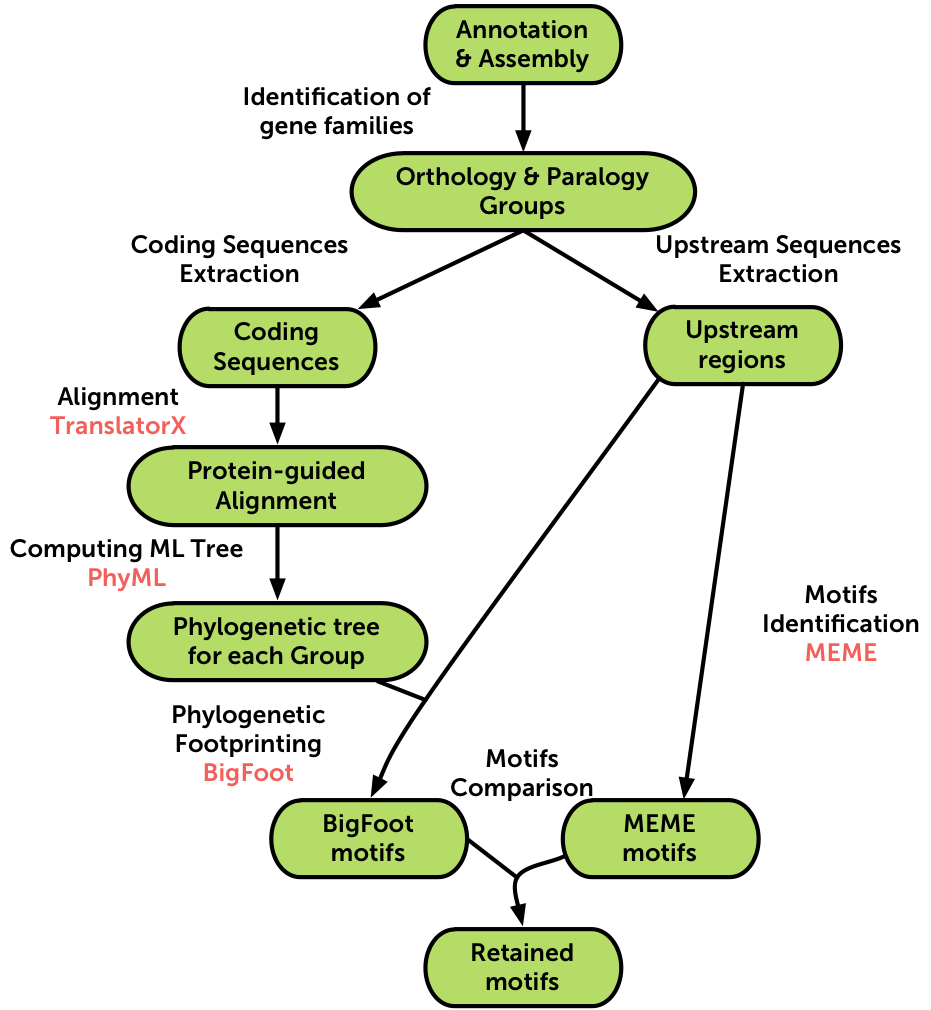
\includegraphics{Figures/Pipeline.png}
\end{center}
\caption{
{\bf Flow chart of the whole pipeline.}  From the genome assembly and annotation of the four species, we used orthology and paralogy groups from \citep{mcgrath_insights_2014}. For each of these families we extracted the coding sequences (CDS) as well as upstream regions from the start codon. We built a maximum likelihood phylogenetic tree using PhyML on pre-aligned CDS with TranslatorX \citep{abascal_translatorx:_2010}. On the one hand we computed the first fifth motifs of size of at least 4 nt using MEME on upstream regions \citep{bailey_meme:_2006}, while on the other hand using both the tree and the upstream sequences were used to detect motifs with a phylogenetic footprinting approach using BigFoot \citep{satija_bigfoot:_2009}. We then retained only conserved motifs between MEME and BigFoot.
}
\label{fig:Pipeline}
\end{figure}

\begin{figure}[!ht]
\begin{center}
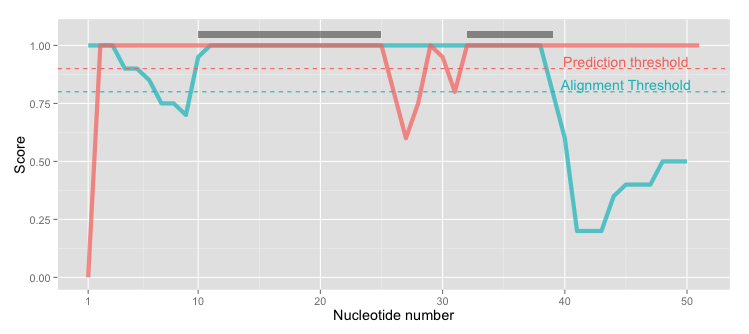
\includegraphics[scale=0.6]{Figures/ScoresPlot.png}
\end{center}
\caption{
{\bf Motif detection from BigFoot example.} BigFoot proceeds to phylogenetic prediction using an alignment technique, refer to~\citep{satija_bigfoot:_2009} for more informations. For each position in the alignment, BigFoot assigns an alignment confidence score and phylogenetic footprinting,\textit{i.e.} motif prediction, confidence score. In our analysis we used a detection technique to allow gaps in both the prediction and the alignment score. Curves: Red solid: Prediction score, Red dashed: Prediction threshold used, Blue solid: Alignment score, Blue dashed: Alignment threshold. Gray boxes: potential motifs detected in the sequence.
}
\label{fig:Scores}
\end{figure}

%\section*{Tables}
%\begin{table}[!ht]
%\caption{
%\bf{Table title}}
%\begin{tabular}{|c|c|c|}
%table information
%\end{tabular}
%\begin{flushleft}Table caption
%\end{flushleft}
%\label{tab:label}
% \end{table}

%\section*{References}
% The bibtex filename
\clearpage
\bibliography{references.bib}

\end{document}

